\documentclass[a4paper]{article}
\usepackage{graphicx}
\usepackage{hyperref}
\usepackage{amsmath}
\usepackage{amssymb}
\usepackage{textcomp}
\usepackage[utf8]{inputenc}
\usepackage[polish]{babel}
\usepackage[T1]{fontenc}
\usepackage{standalone}
\usepackage{array}
% pakiet stosowany do url'i w bibliografii, zamienia odnośniki na ładnie sformatowane
\usepackage{url}
% pakiety służące do numerowania i tworzenia algorytmów
\usepackage{algorithmic}
\usepackage{algorithm}
% redefinicja etykiety nagłówkowej listy algorytmów, domyślna jest po angielsku
\renewcommand{\listalgorithmname}{Spis algorytmów}
\addto\captionspolish{\renewcommand{\figurename}{Fig.}}
\addto\captionspolish{\renewcommand{\refname}{References}}
%\renewcommand{\bibname}{References}
% pakiet do wyliczania skali, przydatny przy dużych obrazkach
\usepackage{pgf}
% pakiet służący do automatycznego sortowania odnośników do bibliografii
\usepackage[sort]{natbib}
% tworzenie listingów
\usepackage{listings}
% tworzenie figur wewnątrz figur
\usepackage{subfig}
% do automatycznego skracania nazw rozdziałów i podrozdziałów używanych w nagłówkach strony by mieściły się w jednej linii
\usepackage[fit]{truncate}
% fancyhdr - ładne nagłówki, definicja wyglądu nagłówka, numery stron będą umieszczane w nagłówku po odpowiedniej stronie
\usepackage{fancyhdr}
\pagestyle{fancy}
%\renewcommand{\chaptermark}[1]{\markboth{#1}{}}
\renewcommand{\sectionmark}[1]{\markright{\thesection\ #1}}
\fancyhf{}
% tutaj ograniczamy szerokość pola w nagłówku zawierającego nazwę rozdziału/podrozdziału do 95% szerokości strony
% redefinicja sposobu prezentacji nazw domyślnie wypisywanych wielkimi literami (np. domyślnie w nagłówku Spis treści będzie miał postać SPIS TREŚCI)
% Uwaga! to może popsuć wielkie litery w ogóle! Jak coś nie działa należy usunąć \nouppercase{} z poniższych definicji
\fancyhead[LO]{\nouppercase{\bfseries{\truncate{.95\headwidth}{\rightmark}}}}
\fancyhead[RE]{\nouppercase{\bfseries{\truncate{.95\headwidth}{\leftmark}}}}
\renewcommand{\headrulewidth}{0.5pt}
\renewcommand{\footrulewidth}{0pt}

% definicja typu prostego wymagana przez pierwsze strony rozdziałów itp.
% powyższe reguły niestety tych stron nie dotyczą, gdyż Latex automatycznie przełącza je pomiędzy fancy a plain
% w tym wypadku eliminujemy nagłówki i stopki na stronach początkowych
\fancypagestyle{plain}{%
 \fancyhead{}
 \fancyfoot{}
 \renewcommand{\headrulewidth}{0pt}
 \renewcommand{\footrulewidth}{0pt}
}

\parskip 0.05in


% makro umożliwiające otaczanie symboli okręgami
\usepackage{tikz}
% brak justowania tekstu (bazą okręgu będzie linia tekstu)
\newcommand*\mycirc[1]{%
  \begin{tikzpicture}
    \node[draw,circle,inner sep=1pt] {#1};
  \end{tikzpicture}}

% pionowe justowanie tekstu, środek okręgu pokrywa się ze środkiem tekstu
\newcommand*\mycircalign[1]{%
  \begin{tikzpicture}[baseline=(C.base)]
    \node[draw,circle,inner sep=1pt](C) {#1};
  \end{tikzpicture}}

% zmiana nazwy twierdzeń i lematów
\newtheorem{theorem}{Twierdzenie}[section]
\newtheorem{lemma}[theorem]{Lemat}

% tworzenie definicji dowodu
\newenvironment{proof}[1][Dowód]{\begin{trivlist}
\item[\hskip \labelsep {\bfseries #1}]}{\end{trivlist}}
% \newenvironment{definition}[1][Definicja]{\begin{trivlist}
% \item[\hskip \labelsep {\bfseries #1}]}{\end{trivlist}}
% \newenvironment{example}[1][Przykład]{\begin{trivlist}
% \item[\hskip \labelsep {\bfseries #1}]}{\end{trivlist}}
% \newenvironment{remark}[1][Uwaga]{\begin{trivlist}
% \item[\hskip \labelsep {\bfseries #1}]}{\end{trivlist}}

% definicja czarnego prostokąta zwyczajowo dodawanego na koniec dowodu
\newcommand{\qed}{\nobreak \ifvmode \relax \else
      \ifdim\lastskip<1.5em \hskip-\lastskip
      \hskip1.5em plus0em minus0.5em \fi \nobreak
      \vrule height0.75em width0.5em depth0.25em\fi}

% poniższymi instrukcjami można sterować co ma być numerowane a co nie i co ma być wyświetlane w spisie treści
% \setcounter{secnumdepth}{3}
% \setcounter{tocdepth}{5}

% definicja czcionki mniejszej niż tiny (domyślnie takiej małej nie ma)
\usepackage{lmodern}
\makeatletter
  \newcommand\tinyv{\@setfontsize\tinyv{4pt}{6}}
\makeatother

% definicja jeszcze mniejszej czcionki
\usepackage{lmodern}
\makeatletter
  \newcommand\tinyvv{\@setfontsize\tinyvv{3.5pt}{6}}
\makeatother

% pakiet do obsługi wielostronicowych tabel
\usepackage{longtable}
\setlength{\LTcapwidth}{\textwidth}

\usepackage[section] {placeins}

\usepackage{multirow}

\usepackage{slantsc}



\begin{document}

\begin{flushright}
{\large \today}
\end{flushright}

\begin{center}



\textsc{\LARGE Intelligent Information Retrieval }\\[1.5cm]

\textsc{\Large Project }\\[0.5cm]

% Title
%\HRule \\[0.4cm]
{ \huge \bfseries Agent with cognitive structure \\[0.4cm] }

%\HRule \\[1.5cm]

% Author and supervisor
\end{center}
\begin{minipage}{0.7\textwidth}
\begin{flushleft} \large
\emph{Authors:}\\
inż. Mateusz Bodziak 131101 IDS, KSDiR\\
inż. Szymon Grocholski 131126 IDS, KSDiR\\

\end{flushleft}
\end{minipage}

\section{Introduction}
The project is about to implement an agent which should learn the rules of the Wumpus World game. The solution will be based on neuron networks.
	
	\subsection{Main idea}
	Our task was to create an agent without a priori knowledge about the game, the 
	environment and rules then train him and check whether he has learnt something.Main idea is to prepare a training set which will be used by a neural network to learn
	 the rules of the world and test is comparing with different network architectures.
	 Main data flow is shown in the Pic.~\ref{pic:flow}. 
	 
	 Everything starts from worldGenerator where the world is being set. The GUI for the game is presented in Pic.~\ref{pic:gui}. The legend is as follows:
	 	\begin{itemize}
				\item red field - Wumpus!
				\item gray field - hole
				\item yellow field - gold
				\item black rectangle - player 
				\item senses are wrote explicite
			\end{itemize}
	 Then we can play the game by our own or let the network take the decisions. 
	 
	 For every move the agent gets -1 pt. For finding gold agent gets 1000 pts and for encountering the Wumpus or a hole gets -1000 pts. After the game we can check the status of points and the game result.
	 
The world is generated in the beginning of every game and is randomly set. Condition is that in the field $(1,1)$ where the player starts there is no gold, Wumpus nor hole. Unfortunately around 10\%  of the maps are unsolvable because of unfortunate placement of Wumpus and holes. The other 90\%  are the maps which are solvable with certain probability. Not all of them are solvable with probability of $100\%$. In many cases the player has 50\% chance of a good move regardless of previous moves and previous senses.
	 
	 
	  \begin{figure}[!h]
		\centering	
		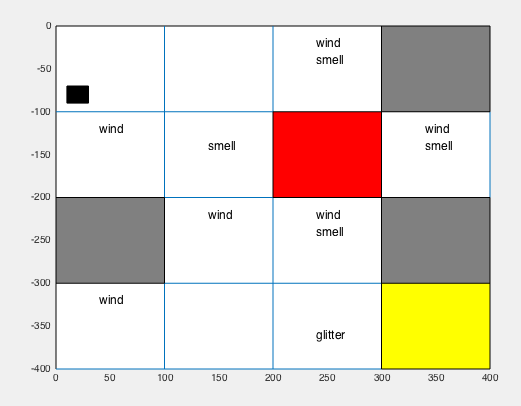
\includegraphics[width=0.9\textwidth]{pic/gui.png}
		\caption{User interface for the Wumpus game}
		\label{pic:gui}
	\end{figure}
	 \begin{figure}[!h]
		\centering	
		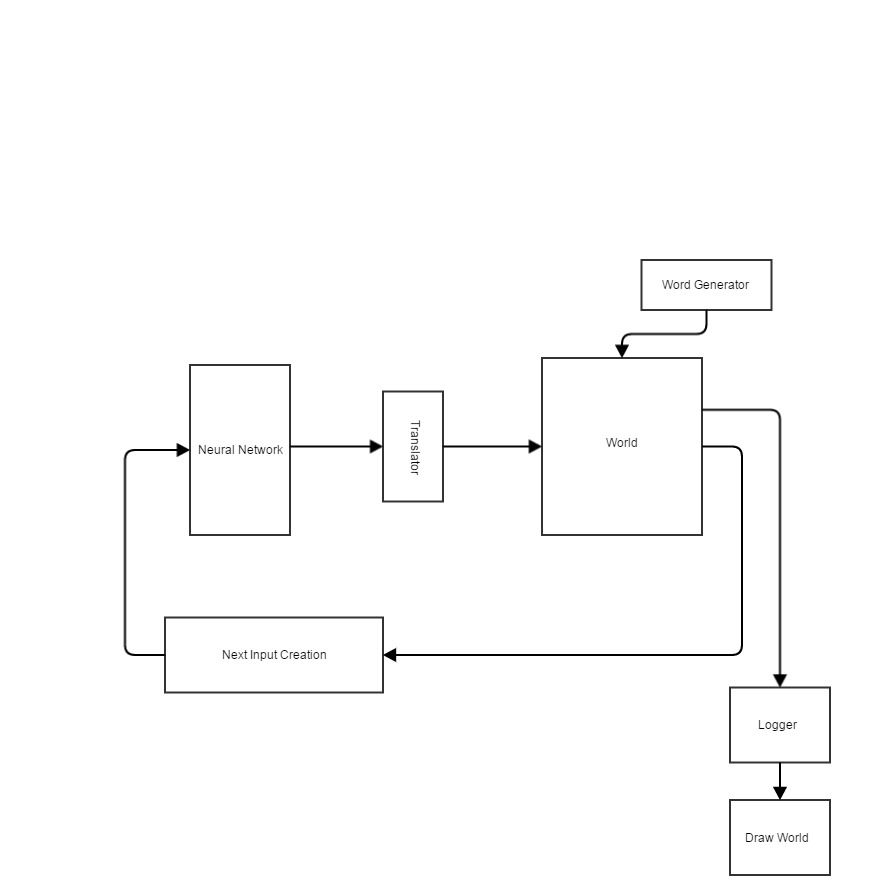
\includegraphics[width=1.2\textwidth]{pic/arch.jpg}
		\caption{Data flow of the program }
		\label{pic:flow}
	\end{figure}

\section{First Approach}
\subsection{Neural Network}
	Our neural network contains parametirized number of hidden layers in testing phase we 
	used 1 and 2 layers. The version with one layer is presented on the Pic~\ref{pic:networkExample}
	\begin{figure}[!h]
		\centering	
		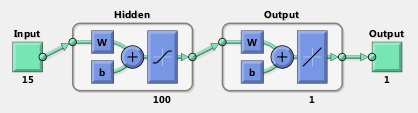
\includegraphics[width=\textwidth]{pic/networkExample.jpg}
		\caption{One of the network architectures}
		\label{pic:networkExample}
	\end{figure}
	
 The input vector is as follows:
	$$
		[x_i, y_i, senses(i), x_(i-1), y_(i-1), senses(i-1), x_(i-2), y_(i-2), senses(i-2)]
	$$
	where 
		$x_i$ - is the current position the row coordinate
		$y_i$ - is the current position the column coordinate
		$senses(i)$ - is a vector of senses from field with coordinates $(x_i, y_i)$
		rest of the coefficients are analogical from previous steps
	
	The output of the network gives us a number from $0-360$ which is the angle. This value
	is translated to a move according to the Pic.~\ref{pic:compass}
	\begin{figure}[!h]
	\centering	
	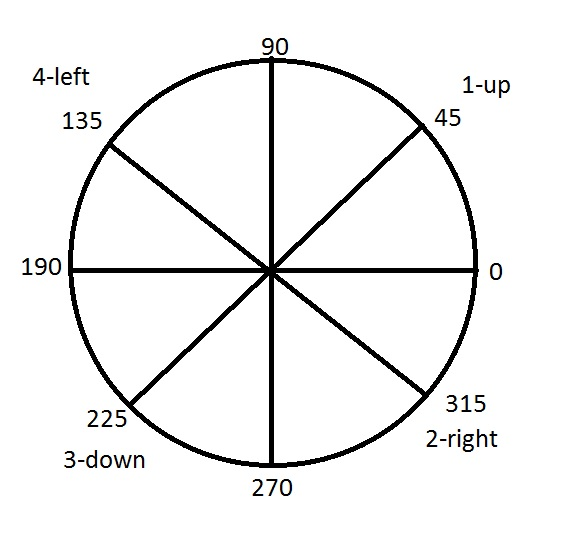
\includegraphics[width=0.7\textwidth]{pic/kompass.jpg}
	\caption{The picture shows how angles are mapped into move}
\label{pic:compass}
\end{figure}
	\begin{itemize}
		\item 1 - UP
		\item 2 - RIGHT
		\item 3 - DOWN
		\item 4 - LEFT
	\end{itemize}
	

\subsection{Implementation }
		\begin{enumerate}
		\item Training data preparation
			\begin{itemize}
				\item Manual data generator 
				\item Automated data generator
			\end{itemize}
		\item Network training 
		\item Execution
			\begin{itemize}
				\item Animation of one game
				\item Performance comparison 
			\end{itemize}
	\end{enumerate}
	
	\paragraph{Training data}
	We construct two ways of preparing the training data. First one was automated, prepared 
	based on random walkthroughs from which we select and store only good ones. This method
	 generated walkthroughs with success - gold was found. Unfortunately this method has stored 
	 many moves which had no sense, like bumping often into walls and ignoring the meaning 
	 of the senses.  
	 
	 Improvement of this was to input some a prori knowledge by human, so we created the manual
	 training data generator which stored the walkthroughs which were committed by a real human player.
	 This enabled us to prepare more suitable training set but it was tiresome and time consuming method.
	 
	After every good walkthrough of the given game all the world are stored on the worldList. This list is needed to display the world for debugging purposes and for preparation of the input vector for the network.
	 
	 
	\paragraph{Network training}
	In this stage we use our training date prepared in the previous stage to train the network.
	The concept of the training is presented on Pic.~\ref{pic:trainDataAuto}
	 \begin{figure}[!h]
		\centering	
		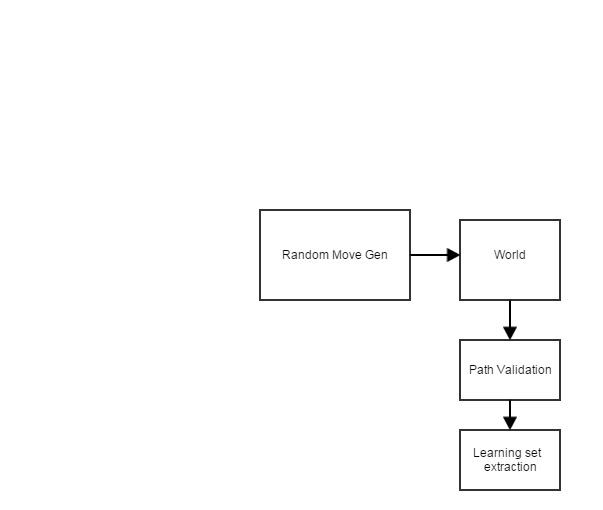
\includegraphics[width=0.7\textwidth]{pic/trainDataAuto.jpg}
		\caption{The algorithm of the training}
		\label{pic:trainDataAuto}
	\end{figure}
	
	\documentclass[a4paper]{article}
\usepackage{graphicx}
\usepackage{hyperref}
\usepackage{amsmath}
\usepackage{amssymb}
\usepackage{textcomp}
\usepackage[utf8]{inputenc}
\usepackage[polish]{babel}
\usepackage[T1]{fontenc}
\usepackage{standalone}
\usepackage{array}
% pakiet stosowany do url'i w bibliografii, zamienia odnośniki na ładnie sformatowane
\usepackage{url}
% pakiety służące do numerowania i tworzenia algorytmów
\usepackage{algorithmic}
\usepackage{algorithm}
% redefinicja etykiety nagłówkowej listy algorytmów, domyślna jest po angielsku
\renewcommand{\listalgorithmname}{Spis algorytmów}
\addto\captionspolish{\renewcommand{\figurename}{Fig.}}
\addto\captionspolish{\renewcommand{\refname}{References}}
%\renewcommand{\bibname}{References}
% pakiet do wyliczania skali, przydatny przy dużych obrazkach
\usepackage{pgf}
% pakiet służący do automatycznego sortowania odnośników do bibliografii
\usepackage[sort]{natbib}
% tworzenie listingów
\usepackage{listings}
% tworzenie figur wewnątrz figur
\usepackage{subfig}
% do automatycznego skracania nazw rozdziałów i podrozdziałów używanych w nagłówkach strony by mieściły się w jednej linii
\usepackage[fit]{truncate}
% fancyhdr - ładne nagłówki, definicja wyglądu nagłówka, numery stron będą umieszczane w nagłówku po odpowiedniej stronie
\usepackage{fancyhdr}
\pagestyle{fancy}
%\renewcommand{\chaptermark}[1]{\markboth{#1}{}}
\renewcommand{\sectionmark}[1]{\markright{\thesection\ #1}}
\fancyhf{}
% tutaj ograniczamy szerokość pola w nagłówku zawierającego nazwę rozdziału/podrozdziału do 95% szerokości strony
% redefinicja sposobu prezentacji nazw domyślnie wypisywanych wielkimi literami (np. domyślnie w nagłówku Spis treści będzie miał postać SPIS TREŚCI)
% Uwaga! to może popsuć wielkie litery w ogóle! Jak coś nie działa należy usunąć \nouppercase{} z poniższych definicji
\fancyhead[LO]{\nouppercase{\bfseries{\truncate{.95\headwidth}{\rightmark}}}}
\fancyhead[RE]{\nouppercase{\bfseries{\truncate{.95\headwidth}{\leftmark}}}}
\renewcommand{\headrulewidth}{0.5pt}
\renewcommand{\footrulewidth}{0pt}

% definicja typu prostego wymagana przez pierwsze strony rozdziałów itp.
% powyższe reguły niestety tych stron nie dotyczą, gdyż Latex automatycznie przełącza je pomiędzy fancy a plain
% w tym wypadku eliminujemy nagłówki i stopki na stronach początkowych
\fancypagestyle{plain}{%
 \fancyhead{}
 \fancyfoot{}
 \renewcommand{\headrulewidth}{0pt}
 \renewcommand{\footrulewidth}{0pt}
}

\parskip 0.05in


% makro umożliwiające otaczanie symboli okręgami
\usepackage{tikz}
% brak justowania tekstu (bazą okręgu będzie linia tekstu)
\newcommand*\mycirc[1]{%
  \begin{tikzpicture}
    \node[draw,circle,inner sep=1pt] {#1};
  \end{tikzpicture}}

% pionowe justowanie tekstu, środek okręgu pokrywa się ze środkiem tekstu
\newcommand*\mycircalign[1]{%
  \begin{tikzpicture}[baseline=(C.base)]
    \node[draw,circle,inner sep=1pt](C) {#1};
  \end{tikzpicture}}

% zmiana nazwy twierdzeń i lematów
\newtheorem{theorem}{Twierdzenie}[section]
\newtheorem{lemma}[theorem]{Lemat}

% tworzenie definicji dowodu
\newenvironment{proof}[1][Dowód]{\begin{trivlist}
\item[\hskip \labelsep {\bfseries #1}]}{\end{trivlist}}
% \newenvironment{definition}[1][Definicja]{\begin{trivlist}
% \item[\hskip \labelsep {\bfseries #1}]}{\end{trivlist}}
% \newenvironment{example}[1][Przykład]{\begin{trivlist}
% \item[\hskip \labelsep {\bfseries #1}]}{\end{trivlist}}
% \newenvironment{remark}[1][Uwaga]{\begin{trivlist}
% \item[\hskip \labelsep {\bfseries #1}]}{\end{trivlist}}

% definicja czarnego prostokąta zwyczajowo dodawanego na koniec dowodu
\newcommand{\qed}{\nobreak \ifvmode \relax \else
      \ifdim\lastskip<1.5em \hskip-\lastskip
      \hskip1.5em plus0em minus0.5em \fi \nobreak
      \vrule height0.75em width0.5em depth0.25em\fi}

% poniższymi instrukcjami można sterować co ma być numerowane a co nie i co ma być wyświetlane w spisie treści
% \setcounter{secnumdepth}{3}
% \setcounter{tocdepth}{5}

% definicja czcionki mniejszej niż tiny (domyślnie takiej małej nie ma)
\usepackage{lmodern}
\makeatletter
  \newcommand\tinyv{\@setfontsize\tinyv{4pt}{6}}
\makeatother

% definicja jeszcze mniejszej czcionki
\usepackage{lmodern}
\makeatletter
  \newcommand\tinyvv{\@setfontsize\tinyvv{3.5pt}{6}}
\makeatother

% pakiet do obsługi wielostronicowych tabel
\usepackage{longtable}
\setlength{\LTcapwidth}{\textwidth}

\usepackage[section] {placeins}

\usepackage{multirow}

\usepackage{slantsc}



\begin{document}


	\paragraph{Performance comparison}
	In order to compare the performance of the networks we constructed an automated tool that was playing the game using trained network. At the same time a random player was playing the same worlds. After selected number of games we calculated the average score and the success rate. Look Pic.~\ref{pic:performanceComp}.
	 
	 
	 \begin{figure}[!h]
		\centering	
		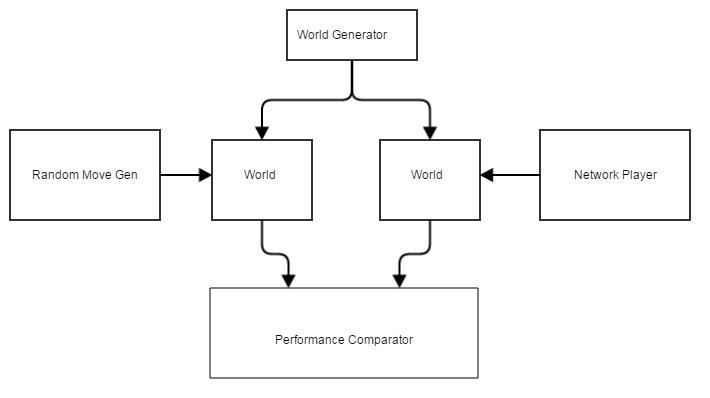
\includegraphics[width=\textwidth]{pic/performance.jpg}
		\caption{Performance comparison}
		\label{pic:performanceComp}
	\end{figure}
	



\end{document}
 

	\subsection{Results}
	\documentclass[a4paper]{article}
\usepackage{graphicx}
\usepackage{hyperref}
\usepackage{amsmath}
\usepackage{amssymb}
\usepackage{textcomp}
\usepackage[utf8]{inputenc}
\usepackage[polish]{babel}
\usepackage[T1]{fontenc}
\usepackage{standalone}
\usepackage{array}
% pakiet stosowany do url'i w bibliografii, zamienia odnośniki na ładnie sformatowane
\usepackage{url}
% pakiety służące do numerowania i tworzenia algorytmów
\usepackage{algorithmic}
\usepackage{algorithm}
% redefinicja etykiety nagłówkowej listy algorytmów, domyślna jest po angielsku
\renewcommand{\listalgorithmname}{Spis algorytmów}
\addto\captionspolish{\renewcommand{\figurename}{Fig.}}
\addto\captionspolish{\renewcommand{\refname}{References}}
%\renewcommand{\bibname}{References}
% pakiet do wyliczania skali, przydatny przy dużych obrazkach
\usepackage{pgf}
% pakiet służący do automatycznego sortowania odnośników do bibliografii
\usepackage[sort]{natbib}
% tworzenie listingów
\usepackage{listings}
% tworzenie figur wewnątrz figur
\usepackage{subfig}
% do automatycznego skracania nazw rozdziałów i podrozdziałów używanych w nagłówkach strony by mieściły się w jednej linii
\usepackage[fit]{truncate}
% fancyhdr - ładne nagłówki, definicja wyglądu nagłówka, numery stron będą umieszczane w nagłówku po odpowiedniej stronie
\usepackage{fancyhdr}
\pagestyle{fancy}
%\renewcommand{\chaptermark}[1]{\markboth{#1}{}}
\renewcommand{\sectionmark}[1]{\markright{\thesection\ #1}}
\fancyhf{}
% tutaj ograniczamy szerokość pola w nagłówku zawierającego nazwę rozdziału/podrozdziału do 95% szerokości strony
% redefinicja sposobu prezentacji nazw domyślnie wypisywanych wielkimi literami (np. domyślnie w nagłówku Spis treści będzie miał postać SPIS TREŚCI)
% Uwaga! to może popsuć wielkie litery w ogóle! Jak coś nie działa należy usunąć \nouppercase{} z poniższych definicji
\fancyhead[LO]{\nouppercase{\bfseries{\truncate{.95\headwidth}{\rightmark}}}}
\fancyhead[RE]{\nouppercase{\bfseries{\truncate{.95\headwidth}{\leftmark}}}}
\renewcommand{\headrulewidth}{0.5pt}
\renewcommand{\footrulewidth}{0pt}

% definicja typu prostego wymagana przez pierwsze strony rozdziałów itp.
% powyższe reguły niestety tych stron nie dotyczą, gdyż Latex automatycznie przełącza je pomiędzy fancy a plain
% w tym wypadku eliminujemy nagłówki i stopki na stronach początkowych
\fancypagestyle{plain}{%
 \fancyhead{}
 \fancyfoot{}
 \renewcommand{\headrulewidth}{0pt}
 \renewcommand{\footrulewidth}{0pt}
}

\parskip 0.05in


% makro umożliwiające otaczanie symboli okręgami
\usepackage{tikz}
% brak justowania tekstu (bazą okręgu będzie linia tekstu)
\newcommand*\mycirc[1]{%
  \begin{tikzpicture}
    \node[draw,circle,inner sep=1pt] {#1};
  \end{tikzpicture}}

% pionowe justowanie tekstu, środek okręgu pokrywa się ze środkiem tekstu
\newcommand*\mycircalign[1]{%
  \begin{tikzpicture}[baseline=(C.base)]
    \node[draw,circle,inner sep=1pt](C) {#1};
  \end{tikzpicture}}

% zmiana nazwy twierdzeń i lematów
\newtheorem{theorem}{Twierdzenie}[section]
\newtheorem{lemma}[theorem]{Lemat}

% tworzenie definicji dowodu
\newenvironment{proof}[1][Dowód]{\begin{trivlist}
\item[\hskip \labelsep {\bfseries #1}]}{\end{trivlist}}
% \newenvironment{definition}[1][Definicja]{\begin{trivlist}
% \item[\hskip \labelsep {\bfseries #1}]}{\end{trivlist}}
% \newenvironment{example}[1][Przykład]{\begin{trivlist}
% \item[\hskip \labelsep {\bfseries #1}]}{\end{trivlist}}
% \newenvironment{remark}[1][Uwaga]{\begin{trivlist}
% \item[\hskip \labelsep {\bfseries #1}]}{\end{trivlist}}

% definicja czarnego prostokąta zwyczajowo dodawanego na koniec dowodu
\newcommand{\qed}{\nobreak \ifvmode \relax \else
      \ifdim\lastskip<1.5em \hskip-\lastskip
      \hskip1.5em plus0em minus0.5em \fi \nobreak
      \vrule height0.75em width0.5em depth0.25em\fi}

% poniższymi instrukcjami można sterować co ma być numerowane a co nie i co ma być wyświetlane w spisie treści
% \setcounter{secnumdepth}{3}
% \setcounter{tocdepth}{5}

% definicja czcionki mniejszej niż tiny (domyślnie takiej małej nie ma)
\usepackage{lmodern}
\makeatletter
  \newcommand\tinyv{\@setfontsize\tinyv{4pt}{6}}
\makeatother

% definicja jeszcze mniejszej czcionki
\usepackage{lmodern}
\makeatletter
  \newcommand\tinyvv{\@setfontsize\tinyvv{3.5pt}{6}}
\makeatother

% pakiet do obsługi wielostronicowych tabel
\usepackage{longtable}
\setlength{\LTcapwidth}{\textwidth}

\usepackage[section] {placeins}

\usepackage{multirow}

\usepackage{slantsc}



\begin{document}


\begin{table}[!ht]
\caption{Networks based on 'randomized' training data PRZYPISSSSSSSSS}
\label{tab:randomizeNetwork}
\begin{center}
\begin{tabular}{|c||l|l|l|l|}
\hline  Num of Neurons & Avg Score & Success Rate& Random Avg Points&Random Success Rate \\ \hline \hline

80 & $-259.72$ &$0.17$&$-588.03$&$0.18$\\
100 & $-467.25$ &$0.21$&$-580.02$&$0.17$\\\hline
\end{tabular}
\end{center}
\end{table}


%\hline  Number of neurons & Avrage Points & Success ratio \hline


\end{document}

\section{Second approach}
	It is clearly visible that the first approach was not one that was promising any improvement. So we decided to rearrange the network. The main issue was that it was hard to provide correct training data. Since we had a framework that was flexible and robust enough we could easily test different configurations of the network.
\subsection{Neural Network project}
\paragraph{Valid moves}
	We found that our network often chooses move that hit the wall so we decided that this is the part of solution that we should focus on. On the pic.~\ref{pic:validMoves} we can see the architecture of the network.

\begin{figure}[!h]
		\centering	
		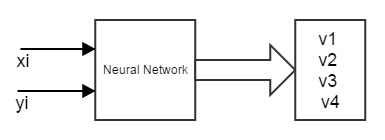
\includegraphics[width=0.7\textwidth]{pic/validMoves.jpg}
		\caption{Valid moves network}
		\label{pic:validMoves}
	\end{figure}
	
	The network returns back a vector of 'validity' of the moves. So each output is a vector $[v1,v2,v3,v4]$ where $vi\in <0,1>$. When the value is $1$ is surely valid when $0$ it is completely not valid.	
\paragraph{Decision Network}
Only avoiding walls was not our goal, so we then thought about a decision making network. Since our last tries consisting three last points were unsuccessful we decided to go witch more local but easier to train controller.

What we noticed is that a network once detects glitter should not diverge more than one field from the point in which the sense was picked.

To make it easier for the network we stated that it is not important if we feel wind or smell since both are equally deadly. So we created a combined sense called 'danger'. Glitter was left intact.

As an input we provided last two senses, last move and current senses (look~\ref{pic:decionMoves}).

\begin{figure}[!h]
		\centering	
		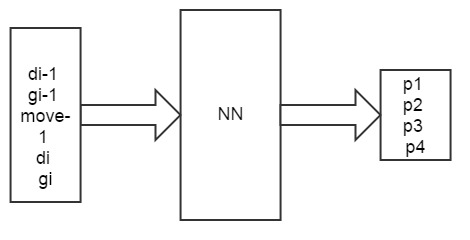
\includegraphics[width=0.7\textwidth]{pic/decisionNet.jpg}
		\caption{The decision network}
		\label{pic:decionMoves}
	\end{figure}

The output was a $4x1$ vector containing probabilities of this move to be chosen by the agent.

\paragraph{Combination}
	The outputs from the network were two $4x1$ vectors. One was representing the validity of the move the second one probability of this move being a good one given current situation.
	
	To combine the two vectors we multiply the value by value. Then normalize the outcome and create 'proportional roulette'. The move that is picked is the move that the agent will take.  

\subsection{Results}
	We encountered a big increase of success ration. Newly created agent was able to win around $31\%$ of games. 
	
	There are still some issues that needs to be addressed.	When an agent doesn't have any memory it may fall into loops that may cause death cause by two many moves. It doesn't know that he has to risk it when there is no other options.

\documentclass[a4paper]{article}
\usepackage{graphicx}
\usepackage{hyperref}
\usepackage{amsmath}
\usepackage{amssymb}
\usepackage{textcomp}
\usepackage[utf8]{inputenc}
\usepackage[polish]{babel}
\usepackage[T1]{fontenc}
\usepackage{standalone}
\usepackage{array}
% pakiet stosowany do url'i w bibliografii, zamienia odnośniki na ładnie sformatowane
\usepackage{url}
% pakiety służące do numerowania i tworzenia algorytmów
\usepackage{algorithmic}
\usepackage{algorithm}
% redefinicja etykiety nagłówkowej listy algorytmów, domyślna jest po angielsku
\renewcommand{\listalgorithmname}{Spis algorytmów}
\addto\captionspolish{\renewcommand{\figurename}{Fig.}}
\addto\captionspolish{\renewcommand{\refname}{References}}
%\renewcommand{\bibname}{References}
% pakiet do wyliczania skali, przydatny przy dużych obrazkach
\usepackage{pgf}
% pakiet służący do automatycznego sortowania odnośników do bibliografii
\usepackage[sort]{natbib}
% tworzenie listingów
\usepackage{listings}
% tworzenie figur wewnątrz figur
\usepackage{subfig}
% do automatycznego skracania nazw rozdziałów i podrozdziałów używanych w nagłówkach strony by mieściły się w jednej linii
\usepackage[fit]{truncate}
% fancyhdr - ładne nagłówki, definicja wyglądu nagłówka, numery stron będą umieszczane w nagłówku po odpowiedniej stronie
\usepackage{fancyhdr}
\pagestyle{fancy}
%\renewcommand{\chaptermark}[1]{\markboth{#1}{}}
\renewcommand{\sectionmark}[1]{\markright{\thesection\ #1}}
\fancyhf{}
% tutaj ograniczamy szerokość pola w nagłówku zawierającego nazwę rozdziału/podrozdziału do 95% szerokości strony
% redefinicja sposobu prezentacji nazw domyślnie wypisywanych wielkimi literami (np. domyślnie w nagłówku Spis treści będzie miał postać SPIS TREŚCI)
% Uwaga! to może popsuć wielkie litery w ogóle! Jak coś nie działa należy usunąć \nouppercase{} z poniższych definicji
\fancyhead[LO]{\nouppercase{\bfseries{\truncate{.95\headwidth}{\rightmark}}}}
\fancyhead[RE]{\nouppercase{\bfseries{\truncate{.95\headwidth}{\leftmark}}}}
\renewcommand{\headrulewidth}{0.5pt}
\renewcommand{\footrulewidth}{0pt}

% definicja typu prostego wymagana przez pierwsze strony rozdziałów itp.
% powyższe reguły niestety tych stron nie dotyczą, gdyż Latex automatycznie przełącza je pomiędzy fancy a plain
% w tym wypadku eliminujemy nagłówki i stopki na stronach początkowych
\fancypagestyle{plain}{%
 \fancyhead{}
 \fancyfoot{}
 \renewcommand{\headrulewidth}{0pt}
 \renewcommand{\footrulewidth}{0pt}
}

\parskip 0.05in


% makro umożliwiające otaczanie symboli okręgami
\usepackage{tikz}
% brak justowania tekstu (bazą okręgu będzie linia tekstu)
\newcommand*\mycirc[1]{%
  \begin{tikzpicture}
    \node[draw,circle,inner sep=1pt] {#1};
  \end{tikzpicture}}

% pionowe justowanie tekstu, środek okręgu pokrywa się ze środkiem tekstu
\newcommand*\mycircalign[1]{%
  \begin{tikzpicture}[baseline=(C.base)]
    \node[draw,circle,inner sep=1pt](C) {#1};
  \end{tikzpicture}}

% zmiana nazwy twierdzeń i lematów
\newtheorem{theorem}{Twierdzenie}[section]
\newtheorem{lemma}[theorem]{Lemat}

% tworzenie definicji dowodu
\newenvironment{proof}[1][Dowód]{\begin{trivlist}
\item[\hskip \labelsep {\bfseries #1}]}{\end{trivlist}}
% \newenvironment{definition}[1][Definicja]{\begin{trivlist}
% \item[\hskip \labelsep {\bfseries #1}]}{\end{trivlist}}
% \newenvironment{example}[1][Przykład]{\begin{trivlist}
% \item[\hskip \labelsep {\bfseries #1}]}{\end{trivlist}}
% \newenvironment{remark}[1][Uwaga]{\begin{trivlist}
% \item[\hskip \labelsep {\bfseries #1}]}{\end{trivlist}}

% definicja czarnego prostokąta zwyczajowo dodawanego na koniec dowodu
\newcommand{\qed}{\nobreak \ifvmode \relax \else
      \ifdim\lastskip<1.5em \hskip-\lastskip
      \hskip1.5em plus0em minus0.5em \fi \nobreak
      \vrule height0.75em width0.5em depth0.25em\fi}

% poniższymi instrukcjami można sterować co ma być numerowane a co nie i co ma być wyświetlane w spisie treści
% \setcounter{secnumdepth}{3}
% \setcounter{tocdepth}{5}

% definicja czcionki mniejszej niż tiny (domyślnie takiej małej nie ma)
\usepackage{lmodern}
\makeatletter
  \newcommand\tinyv{\@setfontsize\tinyv{4pt}{6}}
\makeatother

% definicja jeszcze mniejszej czcionki
\usepackage{lmodern}
\makeatletter
  \newcommand\tinyvv{\@setfontsize\tinyvv{3.5pt}{6}}
\makeatother

% pakiet do obsługi wielostronicowych tabel
\usepackage{longtable}
\setlength{\LTcapwidth}{\textwidth}

\usepackage[section] {placeins}

\usepackage{multirow}

\usepackage{slantsc}



\begin{document}

\section{Performance testing}


Finally we wanted to test our network and compare the results with different kind of players. One of the player was a random player which just choose its move with the probability of 25\% for each direction. The second one was our first approach with one network. Third one was the combained network where we splited the hard task into two simpler taks. Other players are human players with different knowing of the game. The performance was measured by ratio $$performance = \dfrac{won Games}{all Games}$$ and is presented in Table.\ref{tab:performance}.
\begin{table}[!ht]
\caption{Results of the performance of tested players}
\label{tab:performance}
\begin{center}
\begin{tabular}{|c||l|l|l|}
\hline  Player & Won games & All games & Performance  \\ \hline \hline
Random & $1925$ &$10000$ &$19\%$\\
$1^{st}$network & $2132$ & $10000$ &$21\%$\\
Mr Paweł from the train & $21$ &$78$ &$27\%$\\
Szymon & $35$ &$120$ &$29\%$\\
$2^{nd}$combained networks & $3117$ &$10000$ &$31\%$\\
Szymon's Mum & $20$ &$36$ & $56\%$\\

\hline
\end{tabular}
\end{center}
\end{table}

From the results we can assume that the number of 10K games estimates fairly the performance of a random player. That was our minimum goal - to be better than random player. From the results we can easily deduct that splitting the difficult task into two easier tasks was a good idea. The performance is higher than in the first approach. After that we wanted to compare our result to humans. What is really suprising our agent was more effective than most of human players! On the other hand the number of games was different so the results of human players are not accurate enough, although humans during the game are more and more tired and loose their attention so that we assume that the performance in 10000 games could be even worse. Mr Paweł who is a Master of Psychology got 27\%. Nevertheless our agent is the leader except of Szymon's Mum result. In this case we assume that small number of tries could result with bad estimation. 


\end{document}
The human game is presented in~Pic.\ref{pic:humanGame} - the previous senses are visible but the types of fields are hidden.

\begin{figure}[!h]
		\centering	
		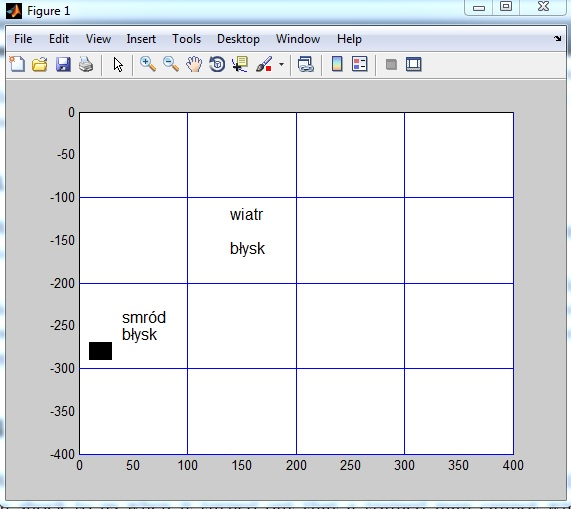
\includegraphics[width=0.7\textwidth]{pic/humanGame.jpg}
		\caption{Human game play}
		\label{pic:humanGame}
	\end{figure}

\section{Summary}

	The problem stated to write an agent with cognitive structure. The knowledge was provided to him in the training of the neuron network. The first approach was not accurate because of the the trainig set, high level of abstraction and too many inputs. The conclusion from second approach is that its better to split the task into two easier tasks. The train data was prepared in better way too which resulted with a good performance. 
This project prepared a good framework for training, testing, and teaching the network how to play a Wumpus game.
\end{document}
